\documentclass{beamer}
\usepackage{listings}
\usepackage{color}
\usepackage{amsmath}
\usepackage{gvv}

\title{Area of Triangle}
\author{EE25BTECH11008 - Anirudh M Abhilash}
\date{October 3, 2025}

\begin{document}

%----------------- Title -------------------
\begin{frame}
\titlepage
\end{frame}

%----------------- Problem -------------------
\begin{frame}{Problem Statement}
Show that the area of the triangle formed by the lines $y=m_1x+c_1$, $y=m_2x+c_2$ and $x=0$ is
\[
\frac{(c_1-c_2)^2}{2\lvert m_1-m_2\rvert}.
\]
\end{frame}

%----------------- Solution -------------------
\begin{frame}{Solution}
Vertices:
\[
\vec{A} = \myvec{0\\c_1}, \quad \vec{B} = \myvec{0\\c_2}.
\]

Intersection of the two lines (RREF):
\begin{align}
\augvec{2}{1}{m_1 & -1 & -c_1 \\ m_2 & -1 & -c_2}
&\xrightarrow{R_2 \leftarrow R_2 - R_1}
\augvec{2}{1}{m_1 & -1 & -c_1 \\ m_2 - m_1 & 0 & -(c_2 - c_1)} \\
&\Rightarrow (m_2 - m_1)x = -(c_2 - c_1) \nonumber \\
&\Rightarrow x^* = \frac{c_2 - c_1}{m_1 - m_2}, \quad y^* = m_1 x^* + c_1.
\end{align}
\end{frame}

%----------------- Solution (cont) -------------------
\begin{frame}{Solution (cont..)}
Vectors:
\[
\vec{u} = \vec{AB} = \myvec{0\\c_2-c_1}, \quad
\vec{v} = \vec{AC} = \myvec{x^*\\y^*-c_1}.
\]

Observe that $y^* - c_1 = m_1 x^*$, hence
\[
\vec{v} = x^* \myvec{1\\m_1}.
\]

Compute norms and dot product:
\begin{align}
\|\vec{u}\|^2 &= (c_2-c_1)^2, \\
\|\vec{v}\|^2 &= x^{*2}(1+m_1^2), \\
\vec{u}\cdot \vec{v} &= (c_2-c_1)(m_1 x^*).
\end{align}
\end{frame}

%----------------- Solution (cont) -------------------
\begin{frame}{Solution (cont..)}
Using $\|\vec{u} \times \vec{v}\|^2 = \|\vec{u}\|^2 \|\vec{v}\|^2 - (\vec{u} \cdot \vec{v})^2$:
\begin{align}
\|\vec{u} \times \vec{v}\|^2 &= (c_2-c_1)^2 x^{*2}(1+m_1^2) - (c_2-c_1)^2 m_1^2 x^{*2} \\
&= (c_2-c_1)^2 x^{*2}.
\end{align}

Thus,
\begin{align}
\|\vec{u} \times \vec{v}\| &= |c_2-c_1|\,|x^*| = |c_2-c_1| \left| \frac{c_2-c_1}{m_1-m_2} \right| \\
&= \frac{(c_2-c_1)^2}{|m_1-m_2|}.
\end{align}
\end{frame}

%----------------- Solution (cont) -------------------
\begin{frame}{Solution (cont..)}
Area:
\begin{align}
\text{Area} &= \tfrac{1}{2} \|\vec{u} \times \vec{v}\| = \frac{(c_1-c_2)^2}{2|m_1-m_2|}.
\end{align}

\[
\boxed{\frac{(c_1-c_2)^2}{2|m_1-m_2|}}
\]
\end{frame}

\begin{frame}[fragile]{Python Code (Plotting Line and Vectors)}
\begin{lstlisting}[language=Python]
import numpy as np
import matplotlib.pyplot as plt

m1, c1 = 1.5, 2 
m2, c2 = -0.5, 5     
A = np.array([0, c1])
B = np.array([0, c2])
x_intersect = (c2 - c1) / (m1 - m2)
y_intersect = m1 * x_intersect + c1
C = np.array([x_intersect, y_intersect])
triangle = np.array([A, B, C, A]) 
\end{lstlisting}
\end{frame}

\begin{frame}[fragile]{Python Code (cont..)}
\begin{lstlisting}[language=Python]
plt.figure(figsize=(6,6))
plt.plot(triangle[:,0], triangle[:,1], 'b-o', label='Triangle')
plt.axvline(0, color='k', linewidth=0.8) 
plt.axhline(0, color='k', linewidth=0.8) 
x_vals = np.linspace(min(0, C[0])-1, max(C[0]+1, 2), 100)
plt.plot(x_vals, m1*x_vals + c1, 'r--', label=f'y={m1}x+{c1}')
plt.plot(x_vals, m2*x_vals + c2, 'g--', label=f'y={m2}x+{c2}')
\end{lstlisting}
\end{frame}

\begin{frame}[fragile]{Python Code (cont..)}
\begin{lstlisting}[language=Python]
plt.scatter([A[0], B[0], C[0]], [A[1], B[1], C[1]], color='black')
plt.text(A[0]-0.3, A[1]+0.1, 'A')
plt.text(B[0]-0.3, B[1]+0.1, 'B')
plt.text(C[0]+0.1, C[1]+0.1, 'C')
plt.grid(True)
plt.axis('equal')
plt.title('Triangle formed by lines and x=0')

plt.show()
\end{lstlisting}
\end{frame}

%----------------- Plot -------------------
\begin{frame}[fragile]{Plot}
\begin{figure}[H]\centering
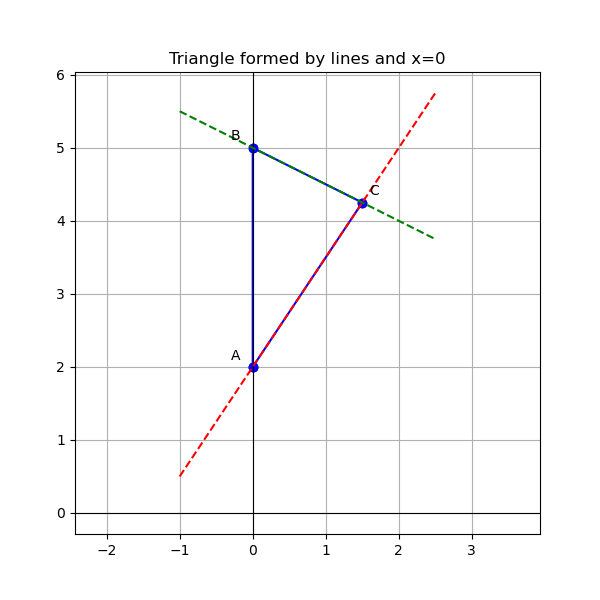
\includegraphics[width=0.8\columnwidth]{figs/plt.png}
\caption{Triangle with example points}
\label{fig:plt}
\end{figure}
\end{frame}

%----------------- C Code -------------------

\begin{frame}[fragile]{C Code (Computations)}
\begin{lstlisting}[language=C]
#include <math.h>

double dot(double* x, double* y, int l) {
    double ans = 0;
    for (int i=0; i<l; i++) {
        ans += x[i]*y[i];
    }
    return ans;
}
\end{lstlisting}
\end{frame}

\begin{frame}[fragile]{C Code (Cont..)}
\begin{lstlisting}[language=C]
double triangle_area(double m1, double c1, double m2, double c2) {
    double A[2] = {0, c1};
    double B[2] = {0, c2};
    
    double x = (c2 - c1) / (m1 - m2);
    double y = m1 * x + c1;
    double C[2] = {x, y};
    
    double u[2] = {B[0] - A[0], B[1] - A[1]};
    double v[2] = {C[0] - A[0], C[1] - A[1]};
    
    double cross = pow(dot(u, u, 2)*dot(v, v, 2) - pow(dot(u, v, 2), 2), 0.5);
    
    return 0.5 * fabs(cross);
}
\end{lstlisting}
\end{frame}


%----------------- Python Code -------------------
\begin{frame}[fragile]{Python Code (Calling C)}
\begin{lstlisting}[language=Python]
import ctypes

lib = ctypes.CDLL("./area.so")

lib.triangle_area.argtypes = [ctypes.c_double, ctypes.c_double, ctypes.c_double, ctypes.c_double]
lib.triangle_area.restype = ctypes.c_double

m1 = float(input("Enter m1: "))
c1 = float(input("Enter c1: "))
m2 = float(input("Enter m2: "))
c2 = float(input("Enter c2: "))

area = lib.triangle_area(m1, c1, m2, c2)
print(f"Triangle area = {area}")
\end{lstlisting}
\end{frame}

\end{document}